\documentclass[12pt]{report}
\usepackage{graphicx}
\usepackage[utf8]{vietnam}
\usepackage[left=3cm, right=3cm, top=3cm, bottom =3cm]{geometry}
\usepackage{pdfpages}
\usepackage{fancybox}
\usepackage{fancyhdr}
\usepackage{hyperref}
\usepackage{etoolbox}
\usepackage{float}
\usepackage{amsmath}
\usepackage{braket}

% \setcounter{tocdepth}{4}

% Link color setup
\hypersetup{
	colorlinks = true,
	linkcolor = black,
	citecolor = blue
}

% Change format of page
\pagestyle{fancy}
\fancyhf{}
\fancyhead{}
\fancyfoot{}
\fancyhead[L]{Toán rời rạc}
\fancyfoot[L]{Nhóm 6 - KSTN-CNTT-K60}
\fancyfoot[R]{\thepage}
\renewcommand{\headrulewidth}{1pt}
\renewcommand{\footrulewidth}{1pt}

\patchcmd{\chapter}{\thispagestyle{plain}}{\thispagestyle{fancy}}{}{}

\renewcommand{\thesection}{\arabic{section}}
\renewcommand{\thesubsection}{\thesection.\arabic{subsection}}
\renewcommand{\thesubsubsection}{\thesubsection.\arabic{subsubsection}}

% format
\usepackage{titlesec}
\usepackage{etoolbox}
\makeatletter
\patchcmd{\ttlh@hang}{\parindent\z@}{\parindent\z@\leavevmode}{}{}
\patchcmd{\ttlh@hang}{\noindent}{}{}{}
\makeatother

\titleformat{\subsection}
{\normalfont\large\bfseries}{\thesubsection}{1em}{}
\titleformat{\subsubsection}
{\normalfont\large\sffamily\bfseries}{\thesubsubsection}{1em}{}

\begin{document}
\thispagestyle{empty}
\thisfancypage{
\setlength{\fboxsep}{0pt}
\fbox}{} 
\begin{center}
\begin{large}

TRƯỜNG ĐẠI HỌC BÁCH KHOA HÀ NỘI
\end{large} \\
\begin{large}
VIỆN CÔNG NGHỆ THÔNG TIN VÀ TRUYỀN THÔNG
\end{large} \\
\textbf{--------------------  *  ---------------------}\\[5.5cm]
{\fontsize{30pt}{1}\selectfont \textbf{BÁO CÁO MÔN HỌC}}\\
{\fontsize{20pt}{1}\selectfont BÀI TẬP LỚN TOÁN RỜI RẠC}\\[5mm]
{\fontsize{18pt}{1}\selectfont CONNECTIVITY IN SENSOR NETWORKS}\\
[2cm]


\begin{tabular}{ r l}
\textbf{Giáo viên hướng dẫn}:& PGS. Huỳnh Thị Thanh Bình\\
\\
\textbf{Nhóm sinh viên thực hiện} :& Tạ Quang Tùng \\ 
 					 		  & Đỗ Tiến Đạt \\
 					          & Nguyễn Minh Quang\\	
 					          & Nguyễn Văn Trung \\
\textbf{Lớp} :& KSTN CNTT K60 \\ 
\end{tabular} 
\vspace{3.7cm}

{\fontsize{14pt}{1}\selectfont  HÀ NỘI}\\
{\fontsize{14pt}{1}\selectfont \today}
\end{center}
\newpage

\tableofcontents
\newpage 

\section{Giới thiệu}
Những năm gần đây đã có sự tăng lên của việc sử dụng mạng sensor để thu thập, đo đạc môi trường. Điều đó đã dẫn đến nhiều những bài toán trong lý thuyết và thực tế về giao thức thu thập và truyền giữ liệu của các sensor.  Ví dụ, mạng sensor có thể được sử dụng để đo đạc mức độ ô nhiễm tại những địa điểm khác nhau trong một khu công nghiệp. Sẽ có những vị trí có mức ô nhiễm cao hơn những vị trí khác. Vì vậy, tại những vị trị khác nhau, tần suất đo đạc, thu lượm dữ liệu của các sensor cũng khác nhau. \cite{somasundara2004mobile}
	
	Dữ liệu được đo đạc bởi các sensor cần phải được chuyển về một trạm  cơ sở (base station) để được xử lý, phân tích. Thông thường, dữ liệu ghi bởi sensor sẽ được truyền về base station thông qua mạng các sensor nối kết nhau. Giải pháp đó là khả thi nhưng dễ dẫn đến hiện tượng quá tải đường truyền tại một số vị trí nào đó (bottleneck). Những sensor ở gần base station sẽ phải chuyển tiếp dữ liệu từ những sensor ở xa gửi đến, đồng thời phải gửi cả dữ liệu của bản thân sensor đó. Điều này dẫn đến những sensor ở gần phải hoạt động với tần suất cao hơn, lượng pin vì thế cũng cạn kiệt nhanh hơn. Hơn nữa, nếu một nút trong mạng hỏng có thể dẫn đến một lượng lớn các sensor không thể gửi dữ liệu về base. Ở một mạng sensor có kích thước lớn, những vấn đề trên càng trở nên khó giải quyết, khó được áp dụng trong thực tế. 
	
	Nhiều những nghiên cứu đã đề xuất giải pháp di động cho vấn đề thu thập dữ liệu. Một phần tử di động, bắt đầu di chuyển từ base station, lần lượt đi qua các sensor trong mạng cảm biến, thu thập dữ liệu của sensor đó, trở về base sau một khoảng thời gian. Bằng giải pháp này, các sensor không cần hình thành một mạng lướng kết nối (ví dụ như một mạng không dây) nên dễ dàng triển khai, tránh được tình trạng bottleneck và một sensor bị hỏng không ảnh hưởng đến sensor khác. 
	
	Có rất nhiều bài toán liên quan đến vấn đề di chuyển của các phần tử di động. Trong bài báo cáo này, chúng em chỉ nghiên cứu về bài toán lập lịch di chuyển trong mô hình \textbf{phần tử di động được điều khiển}. 
	
\section{Phát biểu bài toán}
Một mạng sensor bao gồm các sensor được đặt ở các vị trí khác nhau, thu thập dữ liệu với một tần suất khác nhau. Mỗi sensor có một lượng bộ nhớ lưu trữ tạm thời (buffer) có hạn. Sau một thời gian, buffer sẽ dần dần được lấp đầy dữ liệu. Một phần tử di động bắt đầu di chuyển từ base station, đi qua các nút và thu thập dữ liệu. Khi phần tử di động tiếp cận một sensor và lấy dữ liệu từ nó, dữ liệu của buffer sẽ được xoá bỏ và di chuyển tiếp đến sensor tiếp theo. Sensor sẽ tiếp tục lấp đầy buffer của nó lại từ đầu. Bài toán đặt ra là làm thế nào lập lịch di chuyển của phần tử di động để không một sensor nào trong mạng có buffer bị tràn trong quá trình thu thập. 
\vspace{5mm}

\textbf{Input:} 
\begin{itemize}
\item Một đồ thị vô hướng $G=(V, E)$, $s_0$ là base station, các đỉnh khác là các sensor, và ma trận trọng số $w: E \rightarrow R$ thể hiện thời gian di chuyển của phần tử di động giữa hai đỉnh.
\item Một mảng $overflow\_time: V \rightarrow R$ thể hiện khoảng thời gian lấp đầp buffer của các sensor.  
\item Giá trị $max\_time$ là khoảng thời gian di chuyển lớn nhất của phần tử di động trước khi trở lại base station. 
\end{itemize}

\textbf{Output:} 

Một đường đi $p=\braket{s_0, v_1, v_2, ..., v_k, s_0}$ thoả mãn: 
\begin{enumerate}
\item $\forall v \in V: v \in p$
\item Gọi $travel\_time(v) = \braket{t_1, t_2, ..., t_m}, v \in V$ là các tổng chi phí hoặc khi đi từ $s_0$ đến $v$ lần đầu tiên hoặc đi từ $v$ lần thứ $i$ đến lần thứ $i + 1$ trên đường đi $p$ (giá trị $m$ ứng với mỗi $v$ có thể khác nhau). Thì: 
	$$\forall v \in V, \forall t \in travel\_time(v): t \leq overflow\_time(v) $$
\item Tổng thời gian di chuyển:
	$$w(s_0, v_1) + \sum_{i = 1} ^ {k - 1} w(v_i, v_{i + 1}) + w(v_k, s_0) \leq max\_time$$
\end{enumerate}

\section{Ý tưởng của lời giải bài toán bằng thuật giải di truyền}
\subsection{Những giá trị ảnh hưởng đến quá trình chọn lọc}
Trên thực tế, ta khó có thể tìm được lời giải thoả mãn được điều kiện (1) và (2) hoặc không tồn tại đường $p$ thoả mãn cả 3 điều kiện trên. Thay vào đó, chúng ta sẽ cố gắng tìm lời giải chấp nhận được cho bài toán.

\vspace{5mm}
Gọi:
\begin{itemize}
\item $num\_missed = |V| - |\{v: v \in V, v \in p\}|$ là số lượng các đỉnh chưa được ghé thăm. 
\item $$total\_time = w(s_0, v_1) + \sum_{i = 1} ^ {k - 1} w(v_i, v_{i + 1}) + w(v_k, s_0)$$
\item $$overflow\_rate = \frac{|\{t: \forall v \in V, t \in travel\_time(v), t \leq overflow\_time(v)\}| }{|\{t: \forall v \in V, t \in travel\_time(v)\}|}$$ là tỉ lệ tràn buffer trong quá trình di chuyển. 
\end{itemize}

Một lời giải càng phù hợp khi mà $num\_missed$ và $overflow\_rate$ càng nhỏ, đồng thời $total\_time$ càng gần giá trị $max\_time$.
\subsection{Phương pháp lựa chọn đường đi}
Ở mỗi thời điểm, tại vị trí đỉnh $v$ nào đó, phần tử di động phải xác định những đỉnh sẽ phải ghé thăm tiếp theo. Việc quyết định sẽ chọn đỉnh nào chịu ảnh hưởng bởi độ dài quãng đường đến các đỉnh khác (giá trị $w$) và trạng thái hiện tại của các buffer tới các đỉnh đó (buffer bao lâu nữa sẽ đầy). Để đặc trưng mức độ ưu tiên trong lựa chọn đỉnh $u \neq v$ tiếp theo, chúng ta đặt: 
\begin{equation*}
\begin{split}
weighted\_sum(u, v) & = travel\_weight \times  w(v, u) \\
	& + timeout\_weight \times (next\_overflow\_time(u) - current\_time)
\end{split}
\end{equation*}
Trong đó $current\_time$ là thời gian hiện tại đang xét, $next\_overflow\_time(u)$ là thời gian tràn tiếp theo của đỉnh $u$, được tính bởi giá trị $current\_time$ ở lần ghé thăm trước đó và $overflow\_time(u)$. Giá trị $weighted\_sum$ càng nhỏ thì đỉnh $u$ càng có khả năng cao được lựa chọn làm đỉnh ghé thăm tiếp theo. 

Trong lời giải bài toán này, thay vì chỉ xét đến đỉnh kế tiếp, chúng ta sẽ xét thêm đến những đỉnh sau đó và sau đó nữa trên đường đi tiếp theo. Số lượng các bước di chuyển này trong mỗi lần xét được đặc trưng bởi giá trị $num\_lookahead$. Kết hợp với đánh giá $weighted\_sum$ như sau: 

Giá trị $travel\_weight$ và $timeout\_weight$ là khác nhau đối với mỗi bước di chuyển. Giả sử thời điểm đang xét, phần tử di động đang ở đỉnh $x$. Ta xét những đỉnh $u$ kề với $x$, tính giá trị  $weighted\_sum$ sử dụng giá trị thứ nhất của  $travel\_weight$ và $timeout\_weight$, chọn ra nhiều nhất $num\_remains$ cặp $(u, x)$ có giá trị $weighted\_sum(u, x)$ nhỏ nhất. Với mỗi đỉnh $u$, tiếp tục xét những đỉnh $v$ kề với $u$, tính giá trị  $weighted\_sum(v, u)$ sử dụng giá trị thứ hai của  $travel\_weight$ và $timeout\_weight$, chọn ra nhiều nhất $num\_remains$ cặp $(u, v)$ có giá trị $weighted\_sum(v, u) + weighted\_sum(u, x)$ nhỏ nhất. Cứ tiếp tục như vậy, sau $num\_lookahead$ lần lặp, cuối cùng ta chọn được đường $x \rightarrow u \rightarrow v \rightarrow ...$ mà tổng các $weighted\_sum$ nhỏ nhất. Đó chính là đường đi tiếp của phần tử di động. 

Quá trình xét được lặp đi lặp lại cho đến khi tổng thời gian đã di chuyển vượt quá $max\_time$, các đỉnh ở cuối của đường loại bỏ dần dần và thêm đỉnh $s_0$ ở sau cùng cho đến khi tổng thời gian di chuyển $ \leq max\_time$. Có thể dễ dàng thấy, ứng với mỗi giá trị của $travel\_weight$ và $timeout\_weight$ ở các bước di chuyển ta sẽ thu được một đường đi tương ứng. 

\subsection{Mô tả việc lựa chọn đường đi}
Với các giá trị $num\_lookahead = 3$, $num\_remains = 2$, ta có ví dụ sau (giá trị trên mỗi cạnh là $weighted\_sum$): 

\begin{figure}[H]
\caption{Bước di chuyển 1}
\centering
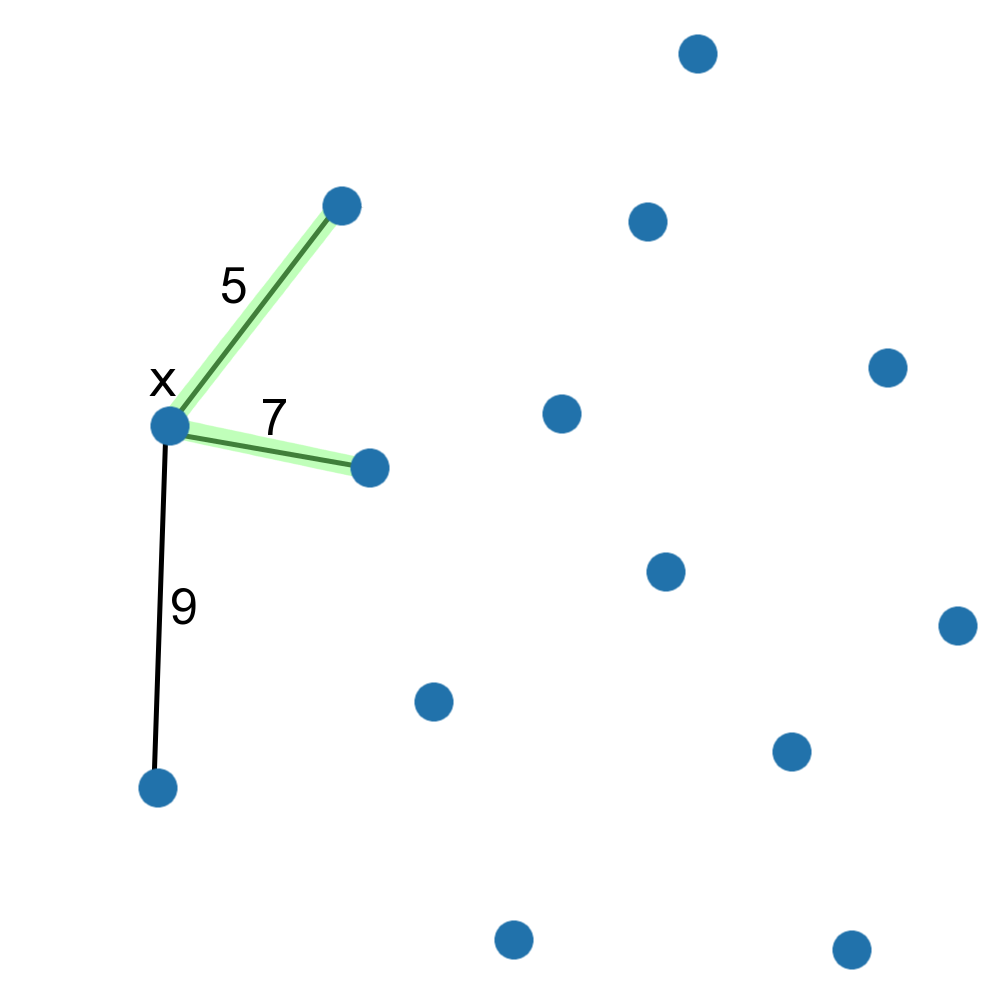
\includegraphics[width=6.5cm]{step-1.png}
\end{figure}

\begin{figure}[H]
\caption{Bước di chuyển 2}
\centering
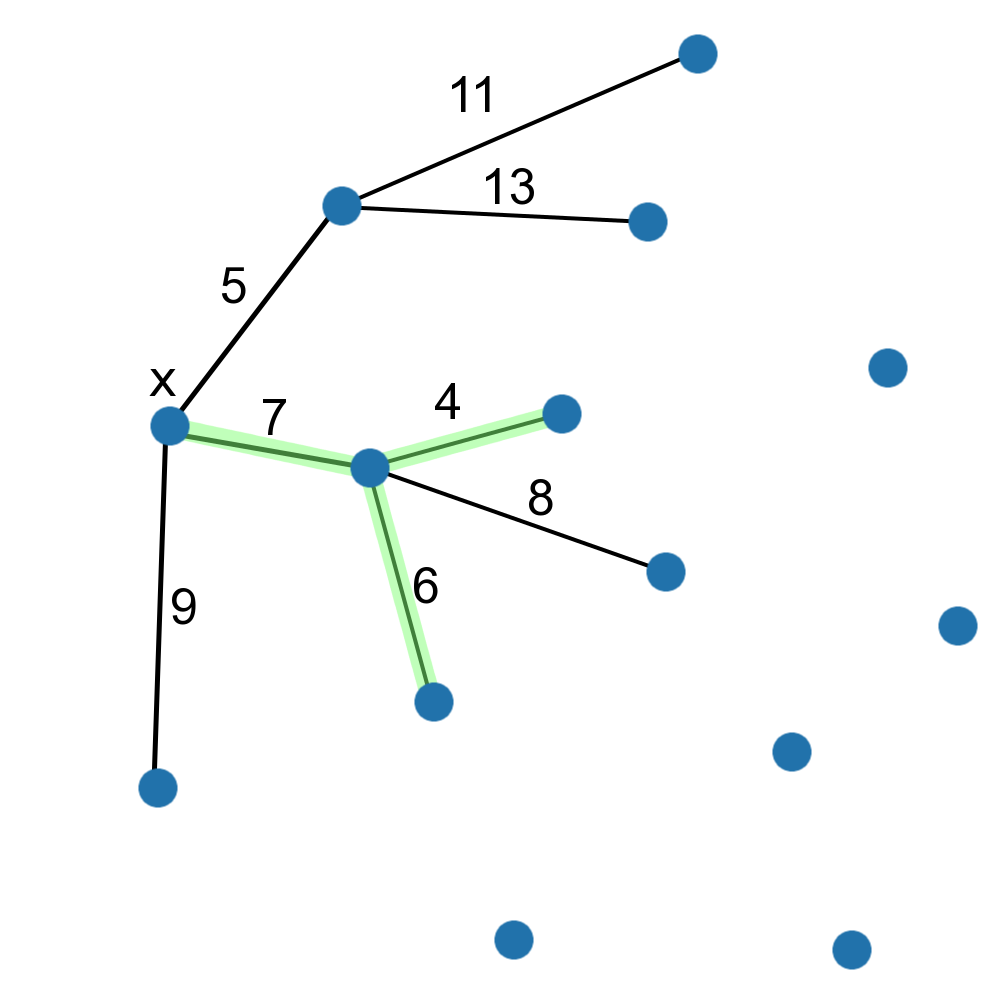
\includegraphics[width=6.5cm]{step-2.png}
\end{figure}

\begin{figure}[H]
\caption{Bước di chuyển 3}
\centering
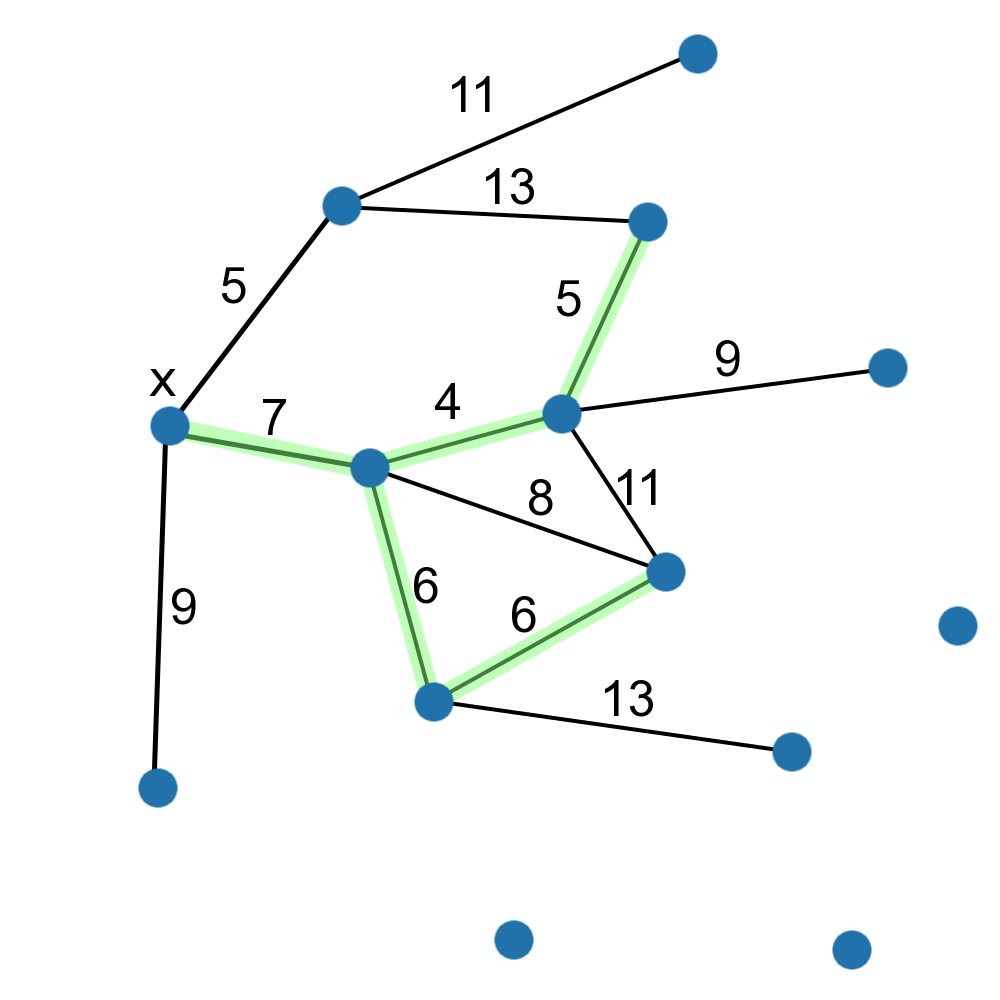
\includegraphics[width=6.5cm]{step-3.png}
\end{figure}

\begin{figure}[H]
\caption{Kết quả cuối cùng}
\centering
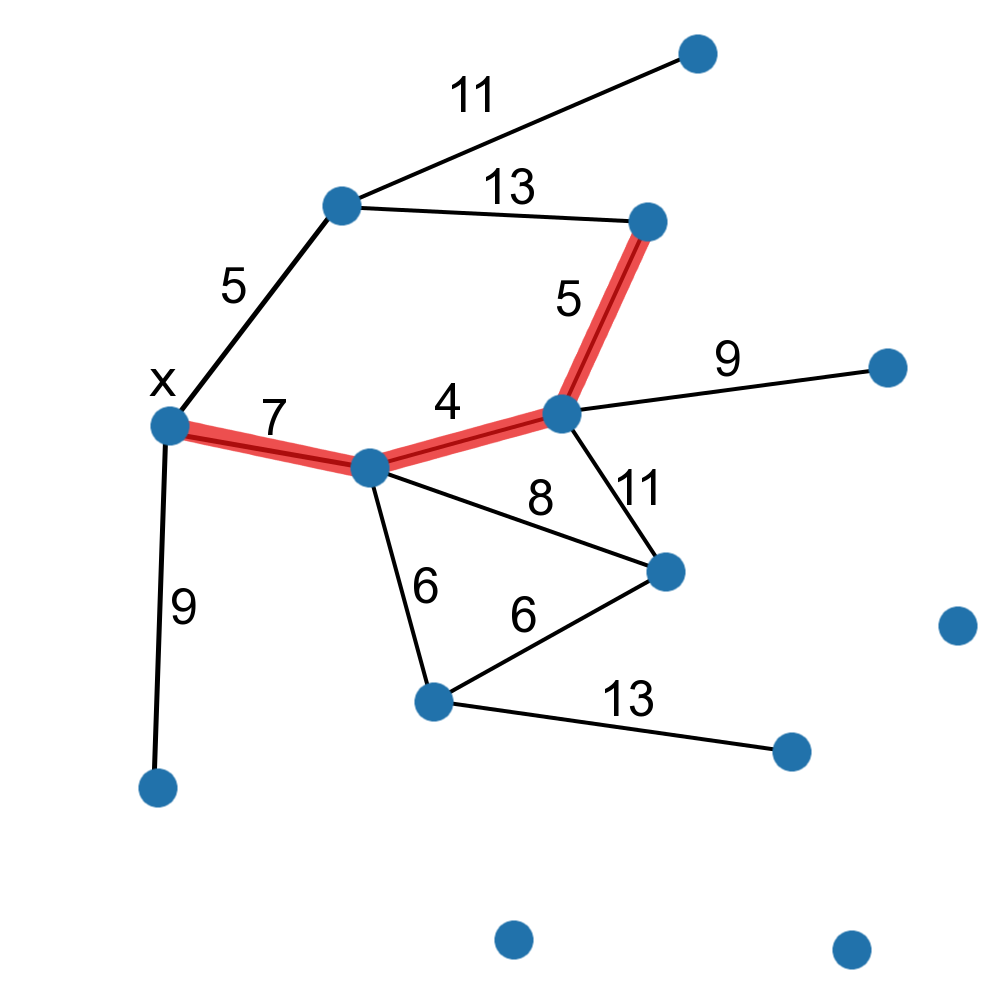
\includegraphics[width=6.5cm]{final.png}
\end{figure}

\subsection{Áp dụng giải thuật di truyền}
Như ở trên, ứng với mỗi giá trị của $travel\_weight$ và $timeout\_weight$ ở các bước di chuyển ta sẽ thu được một đường đi tương ứng. Vì vậy, mỗi cá thể chỉ bao gồm hai mảng $travel\_weight[num\_lookahead]$ và $timeout\_weight[num\_lookahead]$. Đường đi có thể được tính ra nhờ hai mảng đó, từ đó dễ dàng tính được $num\_missed$ và $overflow\_rate$ của đường đi đó. 
Để có quá trình chọn lọc, ta phải có phương pháp đánh giá các cá thể trong quần thể. Cá thể $A$ được cho là tốt hơn cá thể $B$ ( $A < B$) \\
nếu $A.num\_missed < B.num\_missed$ hoặc \\
nếu $A.num\_missed = B.num\_missed$ và $A.overflow\_rate < B.overflow\_rate$

\vspace{10mm}
Gọi $U = \{u_1, u_2, u_3, ..., u_n\}$ là quần thể cần tính toán.   

\subsubsection{Khởi tạo quần thể}
Với mỗi cá thể $u$ trong quần thể, set giá trị $u.travel\_weight[1] = 1$ và các giá trị khác được lấy ngẫu nhiên một số $ \geq 0$.
\subsubsection{Tính toán giá trị fitness}
Với mỗi cá thể $u$ trong quần thể, từ hai mảng $u.travel\_weight$ và $u.timeout\_weight$ ta tìm ra đường đi, từ đường đi ta tính ra các giá trị $u.num\_missed$ và $u.overflow\_rate$.
\subsubsection{Chọn lọc}
Sắp xếp các cá thể trong quần thể $U$ theo thứ tự từ tốt đến kém dần (từ nhỏ đến lớn). Đánh dấu vị trí nào đó ($dead\_index$) mà cá thể từ đó trở đi được coi là đã chết. 
\subsubsection{Lai ghép} 
Với mỗi số nguyên $k \in [dead\_index, n]$, chọn 2 cá thể ngẫu nhiên $u_i, u_j \in U$ thoả mãn $i, j < dead\_index$ và $i \neq j$.  \\
Với mỗi số nguyên $p \in [1,num\_lookahead]$: \\
\hspace*{1cm}$u_k.travel\_weight[p] = crossover(u_i.travel\_weight[p], u_j.travel\_weight[p])$  \\
Với mỗi số nguyên $q \in [1, num\_lookahead]$: \\
\hspace*{1cm}$u_k.timeout\_weight[q] = crossover(u_i.timeout\_weight[q], u_j.timeout\_weight[q])$ 

Trong đó hàm $crossover(a, b)$ thực hiện chuyển $a, b$ thành biểu diễn bit số thực IEEE 32 bit. Chọn ngẫu nhiên một điểm 
chia, kết quả trả về là phần bit thấp của $a$ ghép với phần bit cao của $b$ tính từ điểm chia. 
\subsubsection{Đột biến}
Gọi xác xuất đột biến là $mutation\_prob$. \\
Với mỗi số nguyên $k \in [dead\_index, n]$:	\\
\hspace*{1cm}Với mỗi số nguyên $p \in [1,num\_lookahead]$:	\\
\hspace*{2cm}Chọn ngẫu nhiên số $prob \in [0, 1)$ 	\\
\hspace*{2cm}Nếu $prob \leq mutation\_prob$: $switch\_random\_bit(u_k.travel\_weight[p])$	\\
\hspace*{1cm}Với mỗi số nguyên $q \in [1, num\_lookahead]$: Tương tự như trên. 

Trong đó hàm $switch\_random\_bit(a)$ thực hiện chuyển $a$ thành biểu diễn bit theo kiểu số thực IEEE 32 bit. Chọn ngẫu nhiên $p \in [0, 28]$, đảo bit tại vị trí $p$. 

\section{Kết quả chạy thực tế}
\begin{figure}[H]
\centering
\caption{Vị trí các đỉnh được sinh ngẫu nhiên (đơn vị là theo thời gian)}
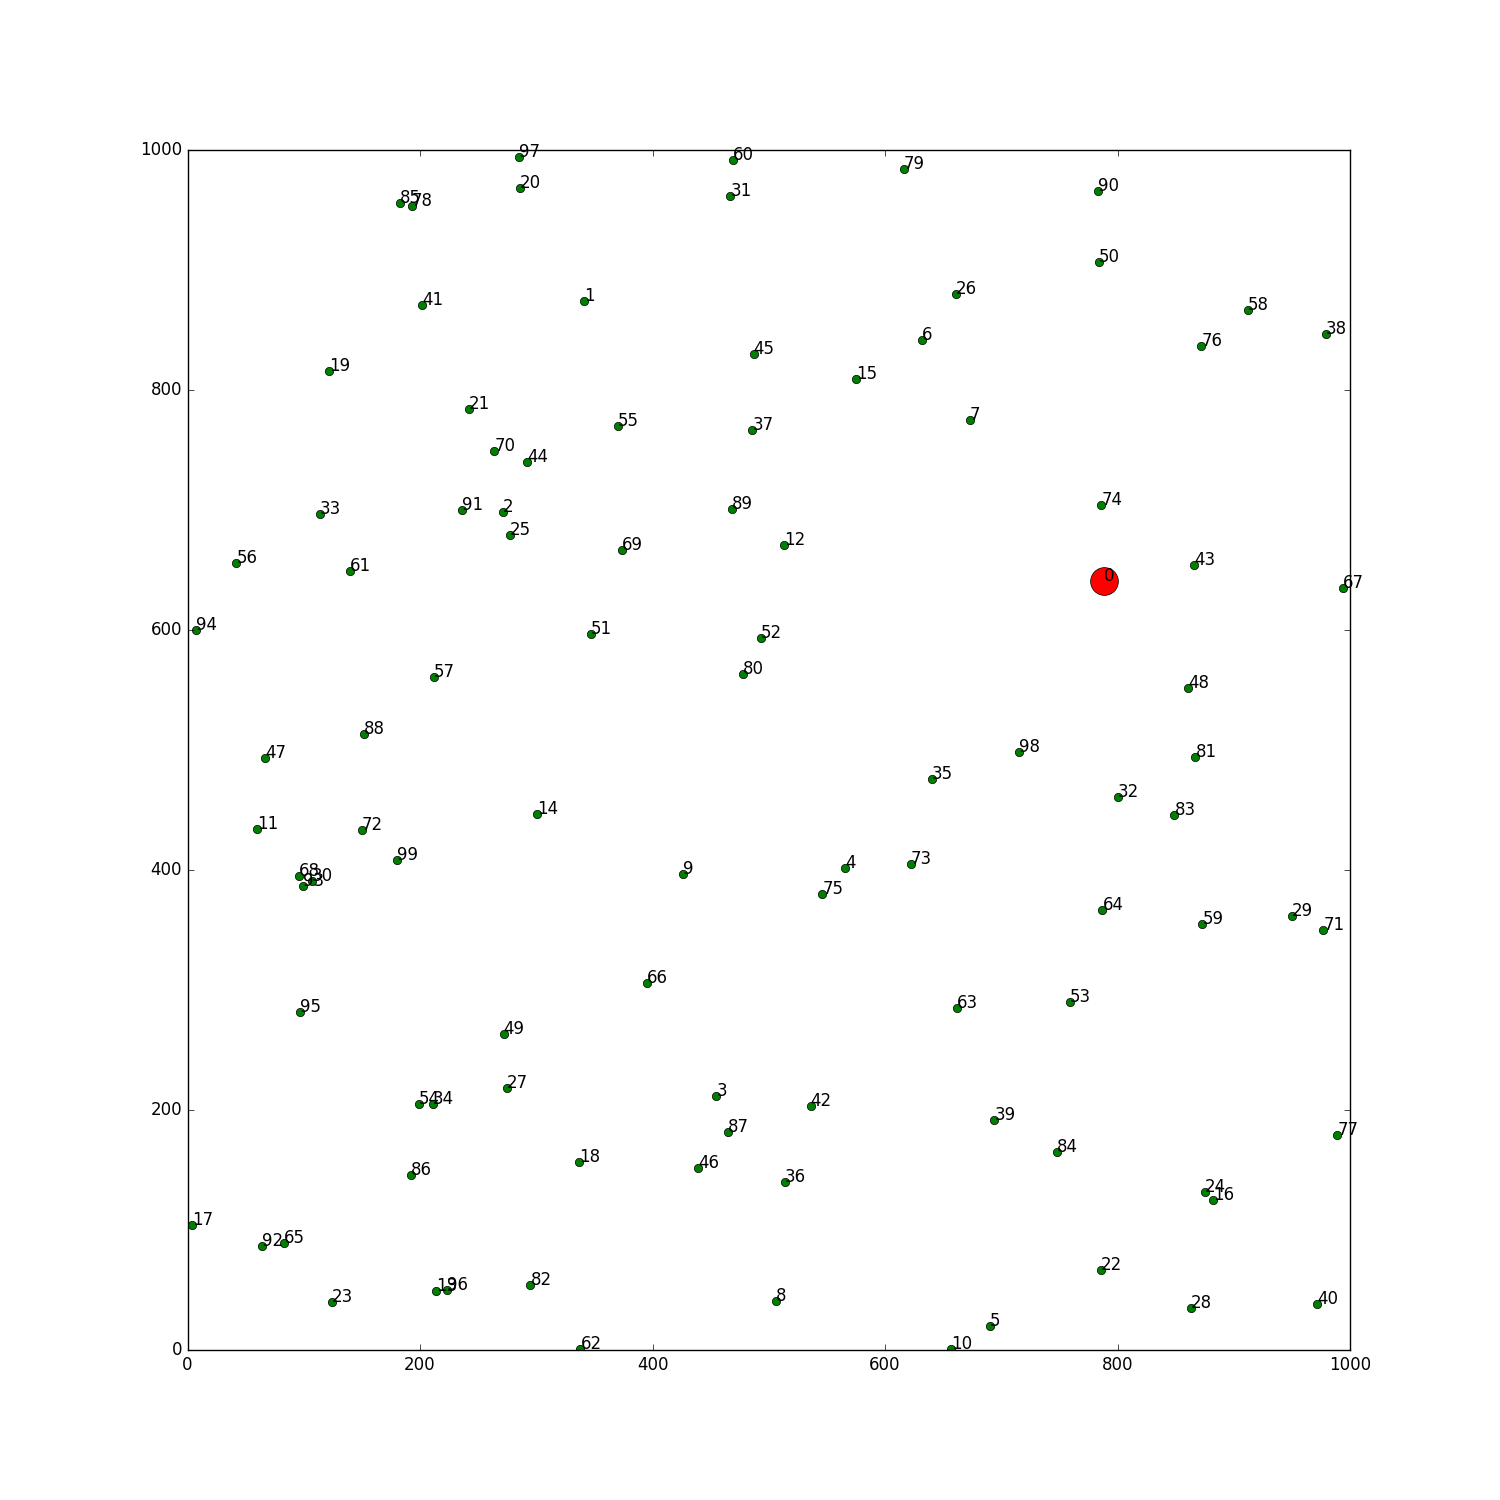
\includegraphics[width=\textwidth]{positions.png}
\end{figure}

\begin{figure}[H]
\centering
\caption{Thời gian tràn của mỗi sensor (Bán kính tỉ lệ thuận với thời gian tràn)}
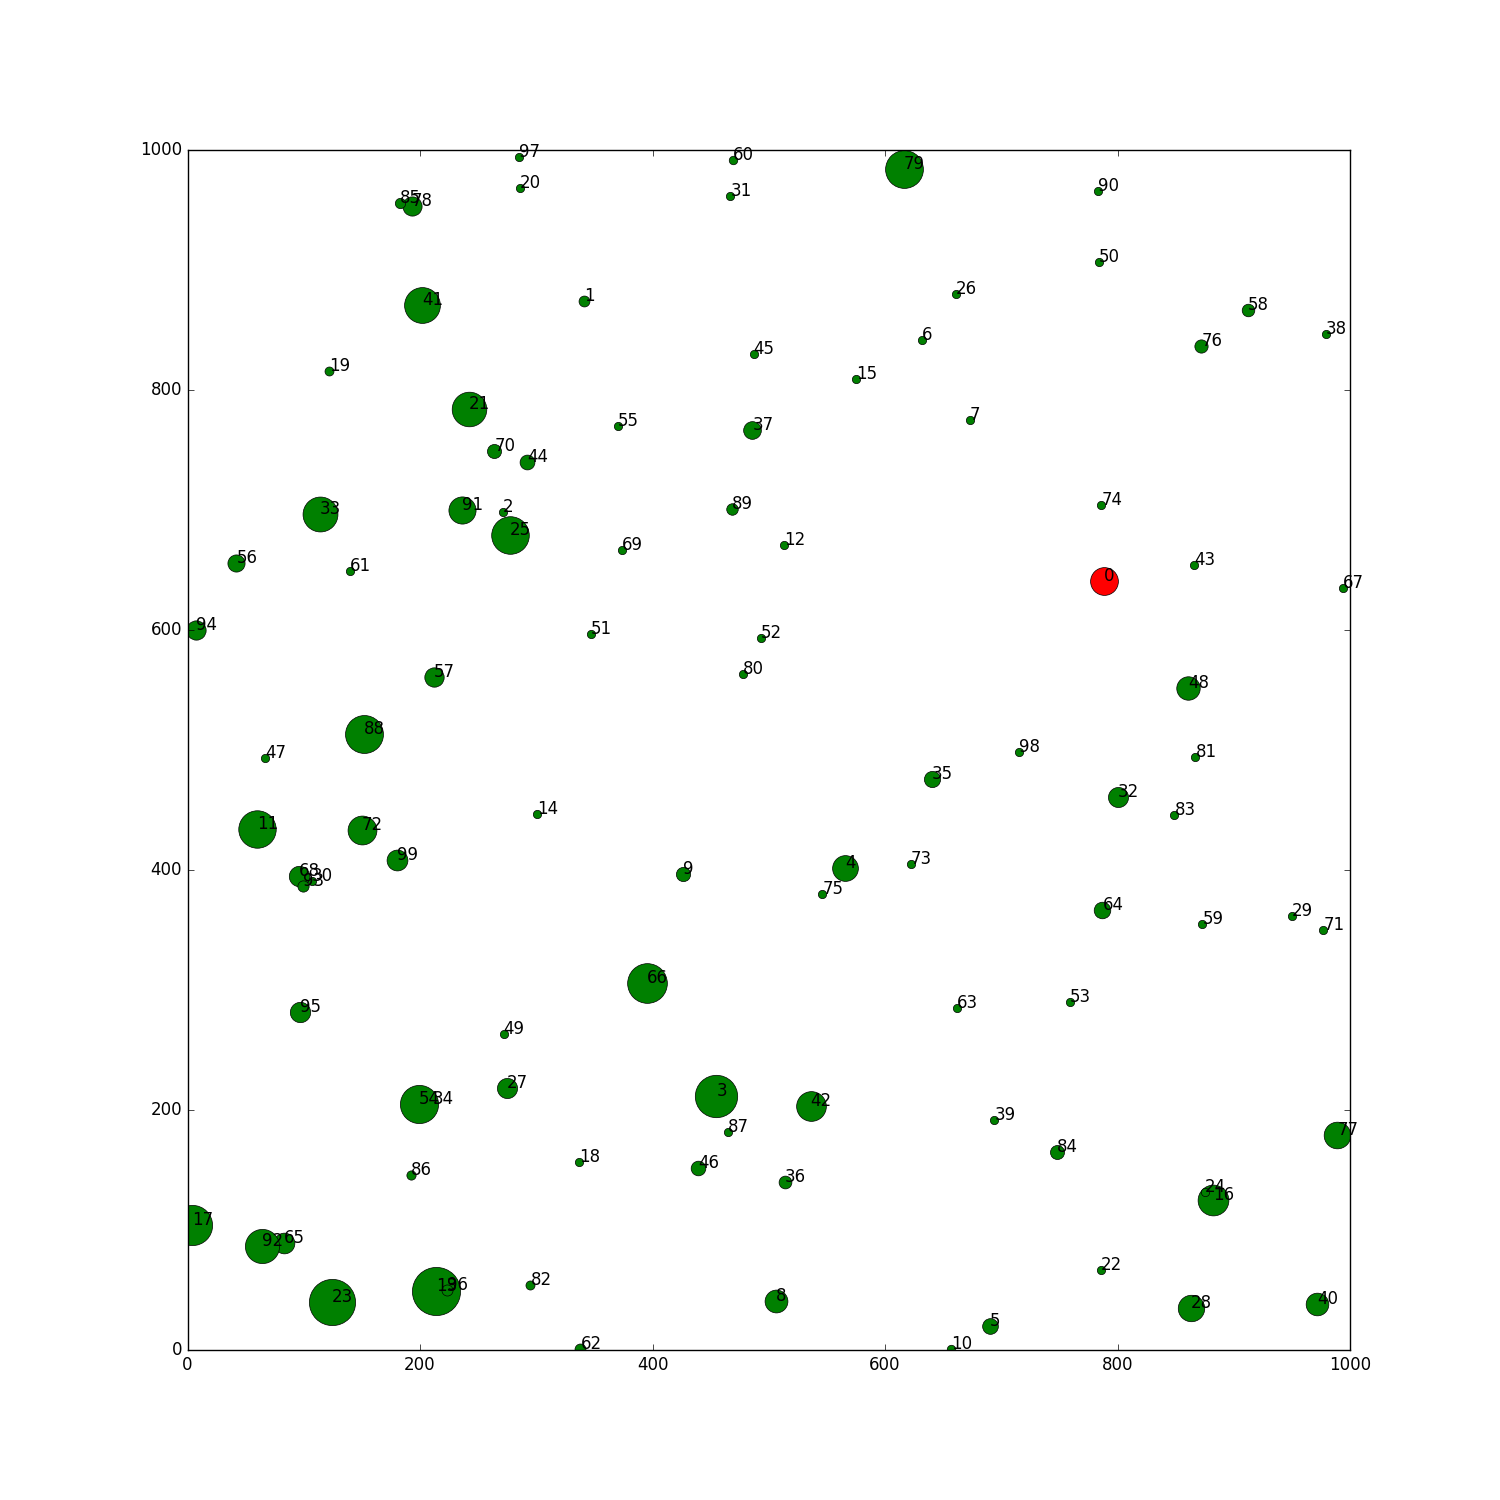
\includegraphics[width=\textwidth]{overflow.png}
\end{figure}

\begin{figure}[H]
\centering
\caption{Đường đi tốt nhất tìm được}
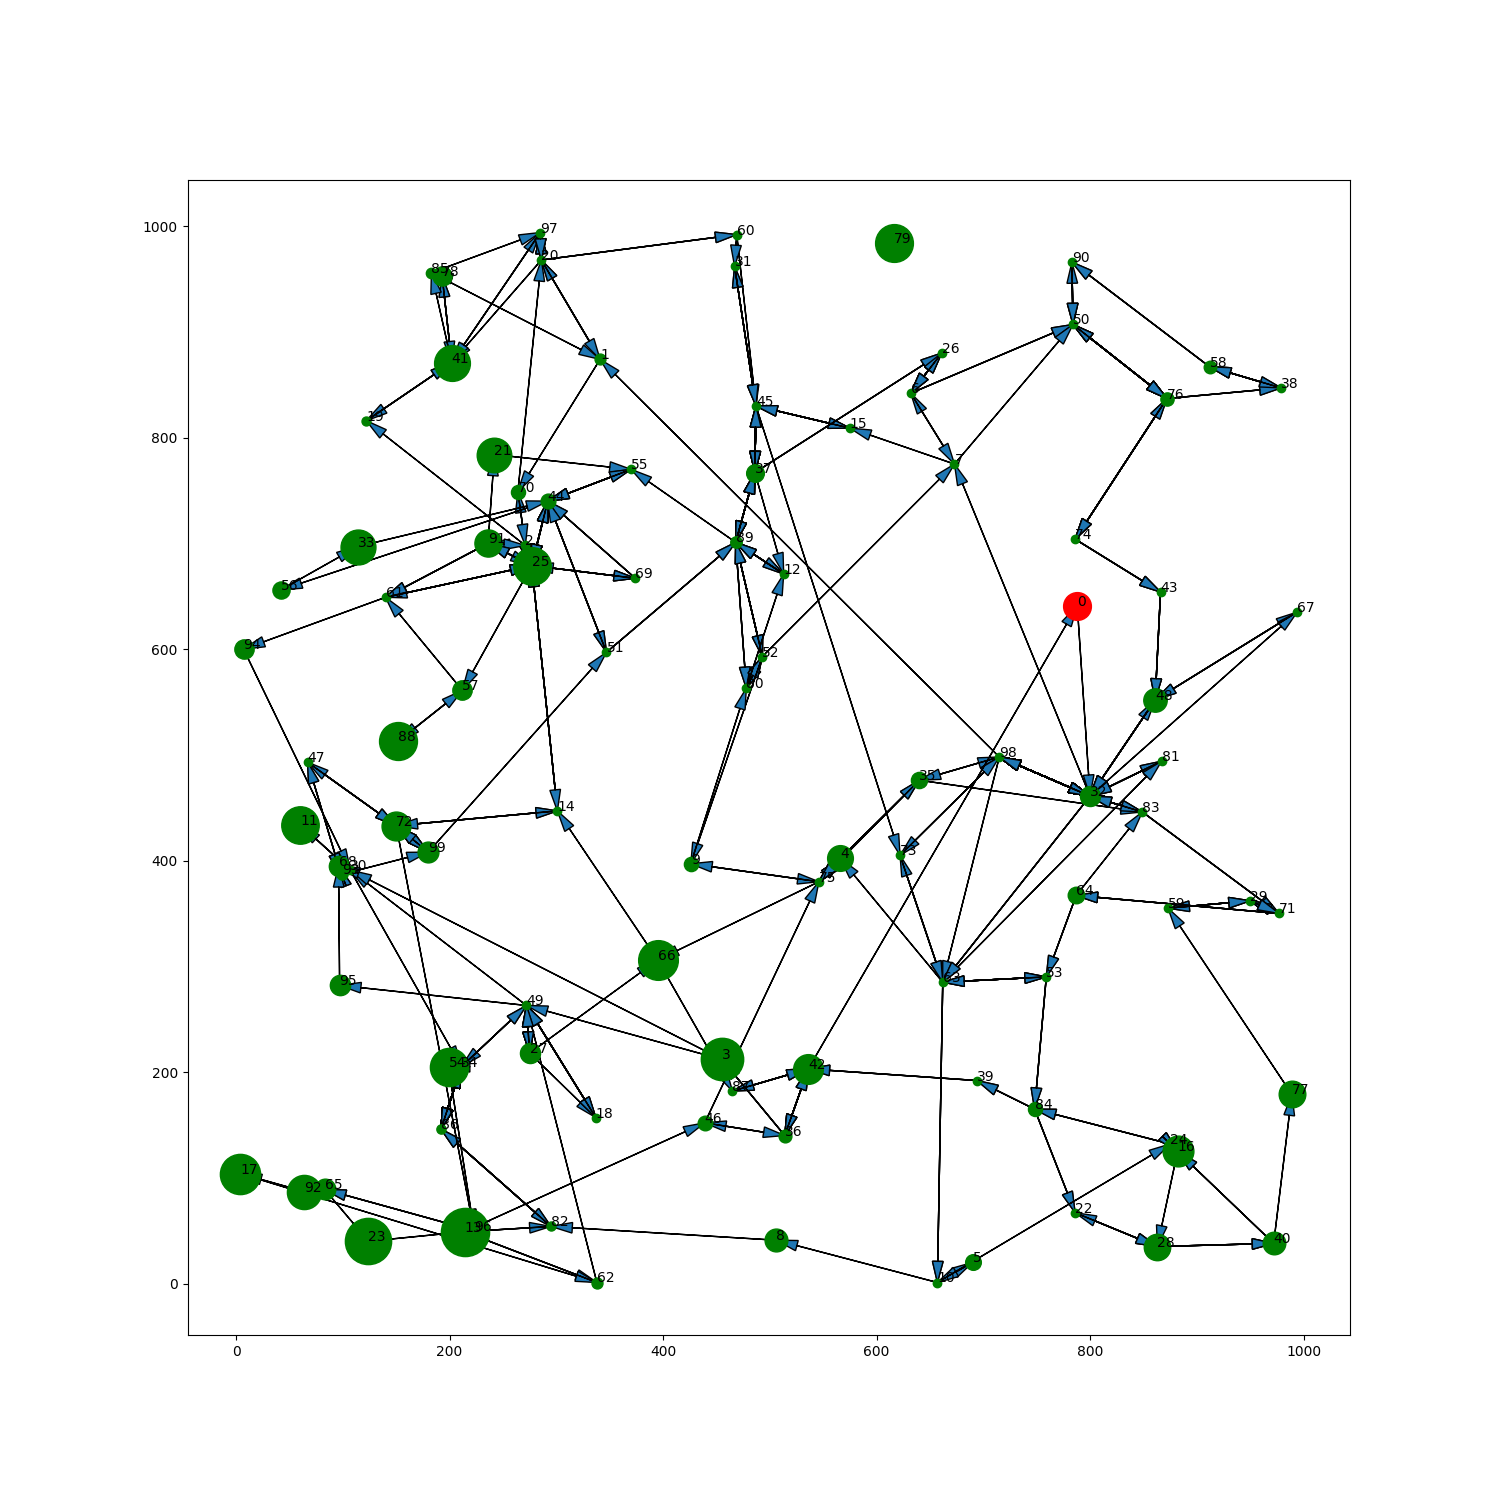
\includegraphics[width=\textwidth]{path.png}
\end{figure}

\begin{figure}[H]
\centering
\caption{Sự tiến hoá của quần thể khi chạy, trong đó \textbf{missed} là $num\_missed$ của cá thể tốt nhất trong quần thể.}
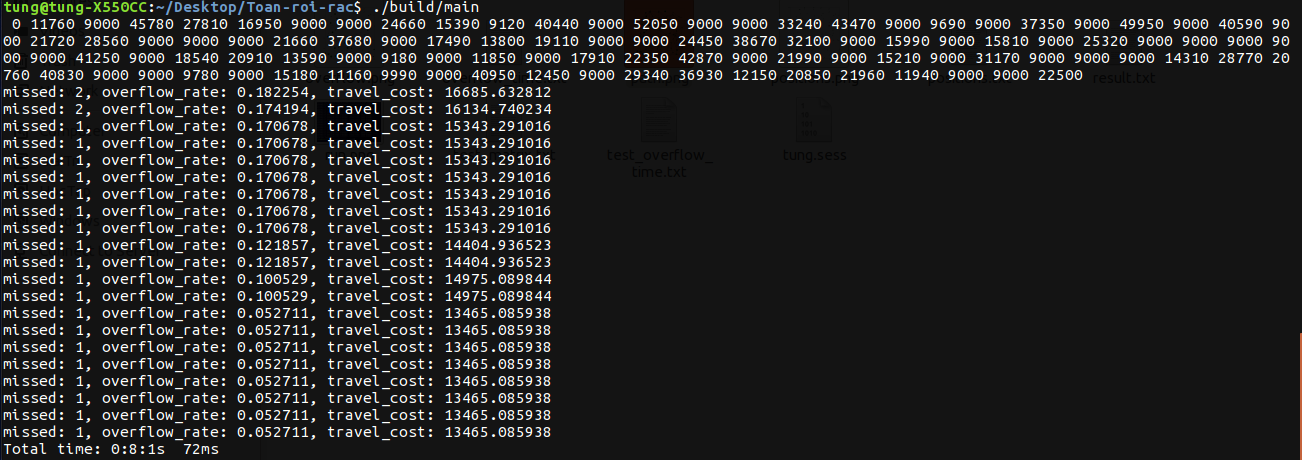
\includegraphics[width=\textwidth]{run.png}
\end{figure}

\section{Hạn chế, tối ưu, cải tiến có thể}
\begin{itemize}
\item Thuật toán chạy với thời gian khá lâu, với 400 cá thể, 100 sensor nhưng đã phải mất 8 phút để thực hiện lặp 20 thế hệ. 
\item Hàm tính toán giá trị fitness có độ phức tạp rất cao, chiếm hơn 99\% tổng thời gian tính của chương trình, cần phải có biện pháp tối ưu hoá tập trung vào hàm này.
\item Chương trình yêu cầu cấp phát động rất thường xuyên, tiêu thụ nhiều bộ nhớ. Có thể cần sử dụng \textbf{pool allocator} để cải tiến tốc độ. 
\item Thuật toán có thể được mở rộng cho trường hợp nhiều phần tử di động. 
\end{itemize}

\begin{thebibliography}{9}

\bibitem{somasundara2004mobile}
  Somasundara, Arun A and Ramamoorthy, Aditya and Srivastava, Mani B,
  \textit{Mobile element scheduling for efficient data collection in wireless sensor networks with dynamic deadlines},
  Real-Time Systems Symposium, 2004. Proceedings. 25th IEEE International, pages 296--305

\end{thebibliography}
\end{document}